\section{Capacitors}

\subsection{capacitors: an introduction}

\subsubsection{capacitors}

\begin{wrapfigure}{r}{6cm}
\centering
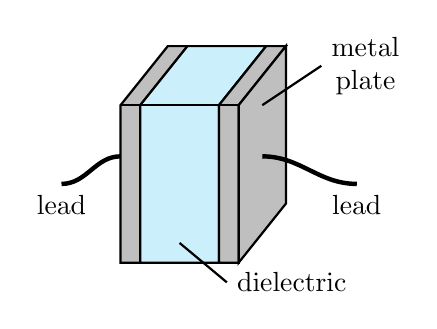
\begin{tikzpicture}[scale=0.5]
\coordinate (A1) at (0,0); 
\coordinate (A2) at (0.5,0);
\coordinate (A3) at (2.5,0); 
\coordinate (A4) at (3,0);
\coordinate (B1) at (0,4); 
\coordinate (B2) at (0.5,4);
\coordinate (B3) at (2.5,4); 
\coordinate (B4) at (3,4);
\coordinate (C1) at (1.2,5.5); 
\coordinate (C2) at (1.7,5.5);
\coordinate (C3) at (3.7,5.5); 
\coordinate (C4) at (4.2,5.5);
\coordinate (D4) at (4.2,1.5);
\draw [thick,fill=gray!50] (A1) -- (A2) -- (B2) -- (C2) -- (C1) -- (B1) -- cycle;
\draw [thick,fill=cyan!20] (A2) -- (A3) -- (B3) -- (C3) -- (C2) -- (B2) -- cycle;
\draw [thick,fill=gray!50] (A3) -- (A4) -- (B4) -- (C4) -- (C3) -- (B3) -- cycle;
\draw [thick,fill=gray!50] (A4) -- (B4) -- (C4) -- (D4) -- cycle;
\draw [thick] (B1) -- (B4);
\draw [ultra thick] (3.6,2.7) [out=0, in=180] to (6,2) node[below]{lead};
\draw [ultra thick] (0,2.7) [out=180, in=0] to (-1.5,2) node[below]{lead};
\draw [thick] (3.6,4) -- ++ (1.5,1) node[right,align=center,execute at begin node=\setlength{\baselineskip}{1.2em}]{metal\\plate};
\draw [thick] (1.5,0.5) -- ++ (1.2,-1) node[right]{dielectric};
\end{tikzpicture}
\vspace*{-20pt}
\end{wrapfigure}

\keypoint{capacitors}\index{capacitor} are elementary electrical units widely used in electrical and electronic engineering

a typical capacitor has two conductive plates

between the plates there is usually an insulating material called \emph{dielectric}

circuit symbol for a capacitor is 
\begin{tikzpicture}[scale=0.2]
\draw (0,0) -- (1.6,0) (2.4,0) -- (4,0);
\draw (1.6,-1) -- (1.6,1) (2.4,-1) -- (2.4,1);
\end{tikzpicture}

\vspace*{\baselineskip}

\begin{wrapfigure}{r}{5.6cm}
\vspace*{-20pt}
\centering
\begin{circuitikz}[european resistors]
	\draw (2,-2) -- (-2,-2)  to[battery,l^=$\mathcal{E}$] (-2,2) -- (-0.5,2);
	\draw (2,-2) -- (2,-2)  to[R,l_=$R$] (2,2) -- (0.5,2);
	\draw (0,-2) -- (0,-1) to[C,l_=$C$] (0,1) -- (0,1.2);
	\draw[fill=white] (0.5,2) circle(0.06) node[above]{$Y$};
	\draw[fill=white] (-0.5,2) circle(0.06) node[above]{$X$};
	\draw[very thick] (0,1.2) --++ (80:1);
	\draw[fill=white] (0,1.2) circle(0.06) node[right]{$S$};
\end{circuitikz}
\end{wrapfigure}

if we construct an electric circuit as shown

when contact $S$ is moved to $X$, capacitor is connected to a voltage supply and becomes charged

positive and negative charges are separated onto two plates, and they will stay where they are even if we disconnect the capacitor from the voltage supply

if we then move $S$ to $Y$, the charged capacitor discharges and drives a current through resistor $R$, i.e., it can act as a temporary power source\footnote{Details on charging and discharging processes will be gone through in \S\ref{sec:charging-capacitors}.}

so capacitors can be used to store and release energy\footnote{Other important functions of capacitors in electronic circuits include smoothing output voltage of power supplies, blocking direct current while allowing alternating current to pass, etc.}


\subsubsection{mutual capacitance}

to describe ability of a capacitor to store charges, we define the notion of capacitance

\begin{ilight}
	\keypoint{(mutual) capacitance}\index{capacitance!mutual capacitance} of a parallel-plate capacitor is defined as the ratio of the charge stored on one plate to the potential difference across the two plates.
\end{ilight}

in a word equation: $\text{mutual capacitance } C = \frac{\text{charge on one plate }Q }{\text{p.d. } V \text{ across the plates}}$ $\quad \Rightarrow \quad$ $\boxed{C = \frac{Q}{V}}$


\cmt unit of capacitance: \keypoint{farad}\index{farad}
\footnote{The unit is named after Michael Faraday, a British physicist who developed the concept of capacitance. Faraday's other main discoveries include electromagnetic induction and electrolysis. He established the basis for the concept of the electromagnetic field in physics.}
: $[C] = \text{F}$

farad a derived unit: $1 \text{ F} = 1 \text{ C}\cdot\text{V}^{-1}$

farad is a large unit, more common subunits of capacitance in use are sub-multiples of farad:

{
	
\centering

$1 \muF = 10^{-6} \text{ F}, \quad 1 \text{ nF} = 10^{-9} \text{ F}, \quad 1 \pF = 10^{-12} \text{ F}$

}

\cmt for a parallel-plate capacitor, charges on the two plates are equal but opposite

net charge on the capacitor: $Q_\text{net} = (+Q)+(-Q)=0$

so we should emphasise on the notion of charge on \emph{one} plate in the definition



\cmt capacitance depends on \emph{geometry} of the device and permittivity of the dielectric material

capacitance does not depend on electric field or potential\footnote{Recall the resistance of an electrical component. Resistance is defined as the ratio of p.d. to current, but the value of resistance is essentially dependent on the length, cross-sectional area and material of the component, instead of the p.d. applied or the current flowing through it.}

for example, capacitance between two metal plates is: $C=\frac{\epsilon_0 A}{d}$
\footnote{If there is \emph{dielectric} in between, the formula should be rewritten as $C = \frac{\epsilon A}{d}$, where $\epsilon$ is permittivity of dielectric. These formulae are not examinable by the syllabus.}

$A$ is area of plate, $d$ is distance between plates, both are geometrical quantities



\subsubsection{self-capacitance}

there are two closely related notions of capacitance: \emph{mutual} capacitance and \emph{self} capacitance

the definition for capacitance given in the previous section, is actually \emph{mutual} capacitance%\footnote{In many cases, the term capactiance is a shorthand for mutual capacitance.}

on the other hand, all bodies are able to store electrical charge

any object that can be electrically charged exhibits capacitance

we define \keypoint{self-capacitance}\index{capacitance!self-capacitance} of an object as the amount of charge that must be added to increase per unit electrical potential

in a word equation, $ \text{self capacitance }C=\frac{\text{charge of object }Q}{\text{electric potential of object }V} \RA \boxed{C=\frac{Q}{V}}$\footnote{For either mutual capacitance or self capacitance, defining equation $C=\frac{Q}{V}$ takes the same form, but you should keep in mind that $Q$ and $V$ represent different things in different contexts.}

\example{Self-capacitance of a charged metal sphere in a vacuum}

consider a metal sphere of radius $R$ and carries an electric charge of $Q$

its electric potential: $V = \frac{Q}{\ec R}$

self-capacitance of the sphere: $C_\text{sphere} = \frac{Q}{V} = Q \times \frac{\ec R}{Q} \RA \boxed{C_\text{sphere} = \ec R}$

note that capacitance is only dependent on its geometrical property (radius $R$) \eoe

\example{A conducting sphere of radius 1.0 m is situated in free space. (a) Find its capacitance. (b) In order to raise its potential to 5000 V, find the amount of charge needed.}

\sol capacitance of the sphere: $C = \ec R = 4\pi\times8.85\times10^{-12}\times 1.0 \approx 1.11\times10^{-10} \text{ F}$

(here you can see farad being an impractically huge unit)

charge on sphere: $Q = CV = 1.11\times10^{-10} \times 5000 \approx 5.56\times 10^{-7} \text{ C}$ \eoe

\subsubsection*{analogy with ideal gases}

an interesting analogy can be made between capacitors and ideal gases

recall an ideal gas is described by equation $pV=nRT$
\footnote{Don't confuse voltage $V$ with volume $V$!}

compare $\left\{\begin{array}{lccl}
\text{amount of charge:} & Q & = &CV \\ \text{amount of substance:} &n & = & \left(\frac{V}{RT}\right) p
\end{array}\right.$

\eqyskip
volume $V$ of a container has a certain space \emph{capacity}, at fixed $T$, pumping more gas (increase $n$) into system, pressure $p$ increases

similarly, a capacitor has a certain charge capacity, adding more charge $Q$ increases p.d. $V$, so the quantity $C$ is naturally called \emph{capacitance}

also for a container, there exists a maximum pressure which it can withstand

for a capacitor, there exists a \emph{breakdown voltage}, or \emph{withstand voltage}, beyond which there could be sparkling across the capacitor

\subsection{energy stored in a capacitor}

to charge a capacitor, need to push electrons off one plate and onto the other

separation of positive and negative charges requires work done $\ra$ energy is stored

\begin{wrapfigure}{l}{5.6cm}
	\vspace*{-8pt}
	\centering
	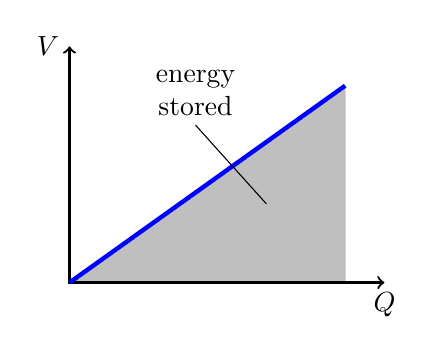
\begin{tikzpicture}[scale=1]
	\draw [gray!50, fill] (0,0) -- (3.5,2.5) -- (3.5,0) -- cycle;
	\draw [thick,<->] (0,3) node[left]{$V$} -- (0,0) -- (4,0) node[below]{$Q$};
	\draw [ultra thick, blue] (0,0) -- (3.5,2.5);
	\draw (2.5,1) -- (1.6,2) node[above,align=center,execute at begin node=\setlength{\baselineskip}{1.2em}]{energy\\stored};
	\end{tikzpicture}
	\vspace*{-16pt}
\end{wrapfigure}

since charge $Q$ varies with p.d. $V$, we shall use the $V$-$Q$ graph to find work done $W$

area under $V$-$Q$ graph is equal to work done $W$

{
	
	\centering
	
	$W = \frac{1}{2} QV$
	
}

substitute $Q=CV$, energy stored in capacitor is\footnote{Rigorously speaking, this electrical potential energy is stored within the \emph{electric fields} between metal plates of capacitor.}:

{

\centering

$\boxed{W = \frac{1}{2}CV^2 = \frac{Q^2}{2C}}$

} 

\example{When the p.d. across a capacitor of $1.8\times10^{-4} \text{ F}$ is increased from 10 V to 20 V, how much additional energy is stored?}

\sol energy change: $\Delta W = W_f - W_i = \frac{1}{2}CV_f^2 - \frac{1}{2}CV_i^2 = \frac{1}{2}\times 1.8\times10^{-4}\times(20^2-10^2) = 2.7\times10^{-2} \text{ J}$ \eoe

\question{A capacitor of 2500 $\muF$ is charged to a working voltage of 18 V. (a) What is the magnitude of positive charge on its plate? (b) What is the energy stored?}

\question{A capacitor initially charged to a potential difference of 16 V discharges and loses 40\% of its energy. What is its new p.d.?}

\question{For an isolated metal sphere of radius 30 cm situated in vacuum, what is the electric potential energy stored when charged to a potential of 120 kV?}


\newpage

\subsection{capacitor networks}

\subsubsection{capacitors in parallel}

\begin{wrapfigure}{r}{6cm}
\vspace*{-20pt}
\centering
\begin{circuitikz}[european resistors,scale=0.9]
\draw (0,0) -- (0,1.6) to[C] (3,1.6) -- (3,0) to[C] (0,0);
\node [below] at (2.1,1.6) {$C_1$};
\node [below] at (0.9,1.6) {$Q_1$};
\node [below] at (2.1,0) {$C_2$};
\node [below] at (0.9,0) {$Q_2$};
\draw (-1,0.8) -- (0,0.8) (3,0.8) -- (4,0.8);
\draw [<->] (0,2.5) -- (1.5,2.5)node[above]{$V$} -- (3,2.5);
\foreach \y  in {0,3} \draw (\y,2.3) -- (\y,2.7);
\end{circuitikz}
\end{wrapfigure}

consider two capacitors connected in parallel

same p.d. $V$ across the network: $V=V_1=V_2$

but charge $Q$ is shared: $Q_\text{total} = Q_1 + Q_2$

{

\centering

$\frac{Q_\text{total}}{V} = \frac{Q_1}{V} + \frac{Q_2}{V}$

$C_\text{total} = C_1 + C_2$

}


if three of more capacitors in parallel: $\boxed{C_\text{total} = C_1 + C_2 + C_3 + \cdots}$ $\quad$ $\boxed{Q_\text{total} = Q_1 + Q_2 + Q_3 + \cdots}$

\cmt adding extra capacitor in parallel to a network, total capacitance will increase

explanation: when several capacitors connected in parallel, equivalent to a single capacitor with larger plates, so more charge on the plates $\ra$ $C\up$

\example{A capacitor with capacitance $C_0$ is charged to a p.d. $V_0$. It is disconnected from the power supply, and then connected across an identical capacitor. Discuss the change in p.d., and change in energy stored in the system.}

\sol initial charge $Q=C_0 V_0$, initial energy stored $W_0 = \frac{1}{2} C V_0^2$

combined capacitance: $C= C_0 + C_0 = 2C_0$

charge is conserved, so final p.d. across: $V = \frac{Q}{C} = \frac{C_0 V_0}{2C_0} = \frac{1}{2} V_0$


charge shared between capacitors, the first capacitor loses half its charge and p.d.

final energy stored in system: $W = \frac{1}{2}CV^2 = \frac{1}{2} \times 2C_0 \times (\frac{1}{2}V_0)^2 = \frac{1}{4} C_0 V_0^2 \ra W = \frac{1}{2} W_0$

half of stored energy is lost as heat when electrons flow between two capacitors \eoe


\question{A capacitor $A$ of capacitance $C$ and a second capacitor $B$ of capacitance $3C$ are connected in parallel. If a voltage is applied across the network, what is the ratio of energy stored in $A$ to that in $B$? What about the ratio of electric charge?}

\newpage

\subsubsection{capacitors in series}

\begin{wrapfigure}{r}{7cm}
\vspace*{-20pt}
\centering
\begin{circuitikz}[european resistors,xscale=0.7]
\draw (0,0) to[C, l_=$C_1$] (4,0) to[C, l_=$C_2$] (8,0);
\node [below] at (2.9,0) {$-Q$};
\node [below] at (1.1,0) {$+Q$};
\node [below] at (6.9,0) {$-Q$};
\node [below] at (5.1,0) {$+Q$};
\draw [<->] (0,1) -- (2,1)node[above]{$V_1$} -- (4,1);
\draw [<->] (4,1) -- (6,1)node[above]{$V_2$} -- (8,1);
\foreach \y  in {0,4,8} \draw (\y,0.8) -- (\y,1.2);
\draw [<->] (0,2) -- (4,2)node[above]{$V$} -- (8,2);
\foreach \y  in {0,8} \draw (\y,1.8) -- (\y,2.2);
\end{circuitikz}
\vspace*{-20pt}
\end{wrapfigure}

consider next two series capacitors

same charge $Q$ on each plate: $Q=Q_1=Q_2$\footnote{Initially, the H-shaped isolated section between capacitors is uncharged. Since no charge can enter or leave this section, its net charge must remain zero, so same charge $Q$ on each plate of series capacitors.}

p.d. is shared: $V_\text{total} = V_1 + V_2$

{
	
	\centering
	
	$\frac{V_\text{total}}{Q} = \frac{V_1}{Q} + \frac{V_2}{Q}$
	
	\eqyskip
	
	$\frac{1}{C_\text{total}} = \frac{1}{C_1} + \frac{1}{C_2} $
	
}


if three of more capacitors in series: $\boxed{\frac{1}{C_\text{total}} = \frac{1}{C_1} + \frac{1}{C_2} + \frac{1}{C_3} + \cdots}$ $\quad$ $\boxed{V_\text{total} = V_1 + V_2 + V_3 + \cdots}$

\cmt adding extra capacitor in series to a network, total capacitance will decrease

explanation: when several capacitors connected in series, equivalent to a parallel-plate capacitor with greater separation, so more charge on the plates $\ra$ $C\down$



\example{For the circuit shown below, find the p.d. across each of the capacitor.}

\begin{figure}[ht]
	\centering
	\vspace*{-12pt}
	\begin{circuitikz}[european resistors,scale=0.8]
		\draw (0,0) to[C,l_=$C_1{=}4.0\text{ }\mu\text{F}$] (3,0) to[C,l_=$C_2{=}12\text{ }\mu\text{F}$] (6,0) -- (6,3) to[battery,l_=$V{=}8.0\text{ V}$] (0,3) -- (0,0);
	\end{circuitikz}
    \vspace*{-12pt}
\end{figure}

\sol using result for combined capacitance, we have: $C_\text{total} = \left( \frac{1}{C_1} + \frac{1}{C_2} \right)^{-1} = \left( \frac{1}{4.0} + \frac{1}{12} \right)^{-1} = 3.0 \text{ }\mu\text{F}$

charge for the network: $Q = C_\text{total} V_\text{total} = 3.0 \times 8.0 = 24 \text{ }\mu\text{C}$

series network so all capacitors have same $Q$, so: $Q_1=Q_2=24 \text{ }\mu\text{C}$

p.d. across each individual capacitor: $V_1 = \frac{Q_1}{C_1} = \frac{24}{4.0} = 6.0 \text{ V}, \quad V_2 = \frac{Q_2}{C_2} = \frac{24}{12} = 2.0 \text{ V}$

alternatively, we can use properties of series network: $Q_1 = Q_2$ and $V_\text{total} = V_1+V_2$

we can solve simultaneous equations: $\left\{\begin{array}{l}
4.0V_1 = 12 V_2 \\
V_1 + V_2 = 8.0
\end{array}\right. \RA 
\left\{\begin{array}{l}
V_1 = 6.0 \text{ V} \\
V_2 = 2.0 \text{ V}
\end{array}\right.$ \eoe



\subsubsection{capacitor networks}

more complicated capacitor networks can be considered as a combination of some smaller networks with capacitors in parallel or in series

\example{$C_1=C_2=C_3=C_4=10\muF$, calculate the capacitance of the network (a) and (b).}\label{ex-Cnet}
\begin{center}
	\vspace*{-8pt}
\begin{minipage}{0.4\linewidth}
\begin{center}
\begin{circuitikz}[european resistors,scale=0.65]
\draw (0,0) -- (0,2) to[C,l^=$C_1$] (2,2) to[C,l^=$C_2$] (4,2) -- (4,0) to[C,l^=$C_3$] (0,0);
\draw (-1,1) -- (0,1) (4,1) -- (5,1);
\end{circuitikz}

\vspace*{-8pt}
(a)
\end{center}
\end{minipage}
\begin{minipage}{0.55\linewidth}
\begin{center}
\begin{circuitikz}[european resistors,scale=0.65]
\draw (0,0) -- (0,2) to[C,l^=$C_2$] (3,2) -- (3,0) to[C,l^=$C_3$] (0,0);
\draw (-3,1) to[C,l^=$C_1$] (0,1);
\draw (3,1) to[C,l^=$C_4$] (6,1);
\end{circuitikz}

\vspace*{-8pt}
(b)
\end{center}
\end{minipage}
\end{center}

\begin{compactitem}
\item[(a)] $C_{12} = \left( \frac{1}{C_1} + \frac{1}{C_2} \right)^{-1} = \left( \frac{1}{10} + \frac{1}{10} \right)^{-1} = 5.0 \muF$

$C_\text{total} = C_{12} + C_3 = 5 + 10 = 15 \muF$

\item[(b)] $C_{23} = C_2 + C_3 = 10 + 10 = 20 \muF$

$C_\text{total} = \left( \frac{1}{C_1} + \frac{1}{C_{23}} + \frac{1}{C_4} \right)^{-1} = \left( \frac{1}{10} + \frac{1}{20} + \frac{1}{10} \right)^{-1} = 4.0 \muF$ \eoe
\end{compactitem}

\example{Four identical capacitors are arranged as shown. Each capacitor can withstand a maximum p.d. of 12 V, what is the maximum safe p.d. to be applied between the terminals?}

\begin{figure}[ht]
	\centering
	\vspace*{-15pt}
	\begin{circuitikz}[european resistors,scale=0.75]
		\draw (0,0) -- (0,2) to[C,l^=$C$] (3,2) -- (3,0) to[C,l^=$C$] (0,0);
		\draw (-3,1) to[C,l^=$C$] (0,1);
		\draw (3,1) to[C,l^=$C$] (6,1);
	\end{circuitikz}
\vspace*{-15pt}
\end{figure}

\sol suppose charge on the leftmost capacitor is $Q$, then charge of rightmost capacitor is also $Q$

but for the two capacitors in parallel, charge is shared, so each has charge $\frac{Q}{2}$

p.d. across the parallel network is half of the p.d. across the two capacitors near the ends

so maximum p.d. across the terminals: $V_\tmax = 12 + 6 + 12 = 30 \text{ V}$ \eoe

\question{Using at most four capacitors of $24 \muF$, design a network that has a combined capacitance of (a) $72 \muF$, (b) $8 \muF$, (c) $36 \muF$, and (d) $18 \muF$.}

\question{If the two networks in Example \ref{ex-Cnet} are both connected to a supply voltage of 15 V, determine the p.d. across each individual capacitor.}


\subsubsection{capacitors \& resistors}

as a quick review, we compare capacitor networks with resistor networks

\begin{center}
{\renewcommand{\arraystretch}{1.2}
\begin{tabular}{|c|c|c|}
\hline
& capacitors & resistors \\ \hline
\multirow{4}{*}{in series}  & same charge & same current \\ [-1ex]
& \multirow{2}{*}{\begin{circuitikz}[european resistors,scale=0.75]
\draw (-0.3,0) -- (0,0) to[C, l^=$C_1$] (2,0) to[C, l^=$C_2$] (4,0) to[C, l^=$C_3$] (6,0) -- (6.3,0) node[right]{$\cdots$};
\end{circuitikz}}  & \multirow{2}{*}{\begin{circuitikz}[european resistors,scale=0.75]
\draw (-0.3,0) -- (0,0) to[R, l^=$R_1$] (2,0) to[R, l^=$R_2$] (4,0) to[R, l^=$R_3$] (6,0) -- (6.3,0) node[right]{$\cdots$};
\end{circuitikz}}  \\
 & & \\ [-1ex]
 & $\frac{1}{C_\text{total}} = \frac{1}{C_1} + \frac{1}{C_2} + \frac{1}{C_3} + \cdots$ & $R_\text{total} = R_1 + R_2 + R_3 + \cdots$ \\ [1.5ex] \hline
\multirow{6}{*}{in parallel}  & same p.d. across & same p.d. across \\ [0ex]
& \multirow{4}{*}{\begin{circuitikz}[european resistors,scale=0.6]
\foreach \x  in {1,2,3} {
\draw (0,6-2*\x) to[C] (4,6-2*\x);
\node[above] at (1.25,6.3-2*\x) {$C_\x$};
}
\draw (-1.5,2) -- (0,2) (4,2) -- (5.5,2);
\draw (0,4) -- (0,0) node[below]{$\vdots$} (4,4) -- (4,0) node[below]{$\vdots$};
\end{circuitikz}}  & \multirow{4}{*}{\begin{circuitikz}[european resistors,scale=0.6]
\foreach \x  in {1,2,3} {
\draw (0,6-2*\x) to[R,l^=$R_\x$] (4,6-2*\x);
}
\draw (-1.5,2) -- (0,2) (4,2) -- (5.5,2);
\draw (0,4) -- (0,0) node[below]{$\vdots$} (4,4) -- (4,0) node[below]{$\vdots$};
\end{circuitikz}}  \\
 & & \\
 & & \\
 & & \\ [0.4ex]
 & $C_\text{total} = C_1 + C_2 + C_3 + \cdots$ & $\frac{1}{R_\text{total}} = \frac{1}{R_1} + \frac{1}{R_2} + \frac{1}{R_3} + \cdots$ \\ [1.5ex] \hline
\end{tabular}}
\end{center}


\newpage

\subsection{charging \& discharging capacitors} \label{sec:charging-capacitors}

in this section, we will investigate how the p.d. across a capacitor changes with time when it is being charged, and we will also look into discharging processes%\footnote{This section is not required by the CIE A-Level exams. However, the contents introduced here may appear in the A-Level syllabus of other examination board.}

\subsubsection{charging phase}

\begin{wrapfigure}{r}{5.4cm}
\centering
\vspace*{-10pt}
	\begin{circuitikz}[european resistors, scale=1.2]
		\draw (0,0) -- (0,3) to[battery,l^=$\mathcal{E}$] (3,3) to[R,l^=$R$] (3,0) to[C,l^=$C$] (0,0);
	\end{circuitikz}
\vspace*{-25pt}
\end{wrapfigure}

	initial state: no charge in capacitor: $Q(0)=0, V_C(0)=0$
	
	at any instant: $\dd Q = C \dd V_C$
		
	current in circuit: $I = \frac{V_R}{R} = \frac{\mathcal{E} - V_C}{R}$
	
	\eqyskip
	change of charge: $\dd Q = I \dd t = \frac{\mathcal{E} - V_C}{R} \dd t = C \dd V_C$
	
	{
	
	\centering
	
	\eqyskip
	$\frac{\dd t}{RC} = \frac{\dd V_C}{\mathcal{E} - V_C}$ 
	
	\eqyskip
	$\int_0^t \frac{\dd t}{RC} = \int_0^{V_C} \frac{\dd V_C}{\mathcal{E} - V_C}$ 
	
	\eqyskip
	$\frac{t}{RC}\Big|_0^t = -\ln(\mathcal{E} - V_C)\Big|_0^{V_C}$

}
			
	simplify everything, we get: $\boxed{V_C = \mathcal{E} \left( 1 - \mathrm{e}^{-t/RC}\right)}$
		
\cmt p.d. of capacitor increases at a decreasing rate when it is being charged

as electric charges are separated onto the two plates, pushing more $+Q$/$-Q$ onto $+\text{ve}$/$-\text{ve}$ plate requires more work done to overcome the repulsion $\ra$ increase in p.d. slows down

\cmt p.d of capacitor eventually tends to the battery e.m.f.

charge will continue to flow if there exists a potential difference

when $V_C = \mathcal{E}$, no charge flow, hence	charging current gradually drops to zero


		
\subsubsection{discharging phase}

capacitor initially charged with $Q(0)=Q, V_C(0) = V_0$
	
at any instant, $\dd Q = -C \dd V_C$ (minus sign because charge decreases during discharging)

\newpage
	
\begin{wrapfigure}{r}{5.4cm}
		\centering
		\vspace*{-12pt}
		\begin{circuitikz}[european resistors, xscale=1.2, yscale=1.5]
			\draw (0,0) -- (0,2) to[C,l^=$C$] (3,2) -- (3,0) to[R,l^=$R$] (0,0);
		\end{circuitikz}
\vspace*{-35pt}
\end{wrapfigure}

	also $V_C=V_R$ because $C$ and $R$ are in parallel
	
	charge change: $\dd Q = I \dd t = \frac{V_C}{R} \dd t = - C \dd V_C$
	
	{
	
	\centering

	\eqyskip
	$- \frac{\dd t}{RC} = \frac{\dd V_C}{V_C}$ 
	
	\eqyskip
	$-\int_0^t \frac{\dd t}{RC} = \int_{V_0}^{V_C} \frac{\dd V_C}{V_C}$
	
	\eqyskip
	$-\frac{t}{RC}\Big|_0^t = \ln(V_C)\Big|_{V_0}^{V_C}$

}
			
	simplify everything, we get: $\boxed{V_C = V_0 \mathrm{e}^{-t/RC} }$
	
\cmt p.d. of capacitor gradually drops to zero during discharging

\cmt discharging current also gradually approaches zero
		
\begin{figure}[ht]
	\centering
	\noindent\begin{minipage}{0.45\linewidth}
		\centering
		\begin{tikzpicture}[xscale=0.9]
		\draw[thick,<->] (0,4) node[left]{$V_C$} -- (0,3.2) node[left]{$\mathcal{E}$} -- (0,0) -- (6,0) node[below]{$t$};
		\draw[thick,dashed] (0,3.2) -- (5.5,3.2);
		\draw [thick,color=blue,domain=0:5.6,samples=12,smooth,variable=\x] plot (\x,{3.2-3.2*exp(-1.2*\x)});
		\end{tikzpicture}
		
		charging phase of capacitor
	\end{minipage}
	\begin{minipage}{0.45\linewidth}
		\centering
		\begin{tikzpicture}[xscale=0.9]
		\draw[thick,<->] (0,4) node[left]{$V_C$} -- (0,3.2) node[left]{$V_0$} -- (0,0) -- (6,0) node[below]{$t$};
		\draw[thick,dashed] (0,3.2) -- (5.5,3.2);
		\draw [thick,color=blue,domain=0:5.6,samples=12,smooth,variable=\x] plot (\x,{3.2*exp(-1.2*\x)});
		\end{tikzpicture}
		
		discharging phase of capacitor
	\end{minipage}
\end{figure}

\subsubsection{time constant}

$\tau \equiv RC$ is called \keypoint{time constant}, which determines charging and discharging rate of a capacitor

$R\up$ $\Rightarrow$ smaller charging/discharging current $\Rightarrow$ takes longer to charge/discharge

$C\up$ $\Rightarrow$ more charge to be charged/discharged $\Rightarrow$ takes longer

charging or discharging of capacitors is not instantaneous, there is always a certain delay

as a rule of thumb, after a time $t=3\sim5\tau$, charging or discharging is almost complete

%time delay for common $RC$ circuits is usually small, but the delay could hinder further increasing of speed in integrated circuits
